\chapter{Introduction}

No matter how powerful a machine, it may not be powerful enough.
This is true of machines that do physical work, but also of machines that compute, as every computer will struggle on some workloads.
When a computational task gets challenging, it is said to be complex.
This is not very precise and indeed, the word \emph{complexity} is used to indicate a wide variety of phenomena.

This thesis introduces a unified framework for the analysis of a multitude of forms of complexity.
A unifying theory need not be better than any of the specific theories it tries to include.
However, it may open the door to new ways of thinking about old concepts and thus enable future developments.

We begin this introductory chapter with an informal section, arguing that there is really no single form of complexity.
This section, Section~\ref{sec:size_of_a_cube}, is intended to be readable by a broad audience and is centered around intuition more than around mathematics.
In Section~\ref{sec:history}, we take a more in-depth look at some of the ways complexity pops up in mathematics and computer science.
The notions of complexity that emerge shall each be subject to an analysis in our unified framework in Chapter~\ref{ch:parameterizations}.
Our unified framework offers a mathematical model of complexity rooted in a branch of computer science called \emph{parameterized complexity theory}.
We shall review the existing formalisms in parameterized complexity theory in Section~\ref{sec:parameterized_complexity_theory}.
A short overview of the contributions presented in this thesis is given in Section~\ref{sec:contributions}.

Following this introductory chapter is a chapter that contains the background theory required for our analysis of multiple forms of complexity.
This background chapter contains two parts.
The first part, Section~\ref{sec:established_theory}, deals with established theory and serves to make this thesis self-contained.
In the second part, Section~\ref{sec:framework}, our new framework for the analysis of complexity is laid out.

The body of this thesis is formed by Chapter~\ref{ch:parameterizations}, which contains all of our results.
It is split into five parts, each dealing with a different form of complexity.
A high-level overview of our results in a shared context is given in Chapter~\ref{ch:conclusion}.


\bigsection{The Size of a Cube}
\label{sec:size_of_a_cube}%

Shown in Figure~\ref{fig:shapes} are three different shapes.
When we ask which of these three shapes is the largest, we start a journey down a deep rabbit hole.
In this thesis, that rabbit hole is explored.
As an indication of what is to come, we briefly consider a comparable question:
What is the largest species of snakes?
The heaviest snakes are anacondas, but the longest snakes are pythons.
Thus, the answer to this question depends on what is meant by \enquote{the largest}.
\begin{figure}[bp]
  % Unit vectors using azimuth a and elevation e:
  % x = ( cos(a), sin(a)sin(e) )
  % y = ( -sin(a), cos(a)sin(e) )
  % z = ( 0, cos(e) )
  % We use an azimuth of 30 degrees and an elevation of 15 degrees.
  % Additionally, we scale the first two figures by 1/cos(a).
  \centering
  \subcaptionbox{A tetrahedron\label{fig:tetrahedron}}[0.3\textwidth]{
    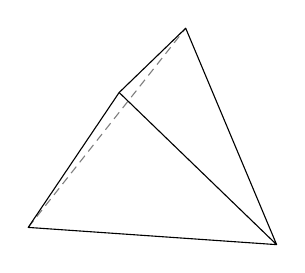
\begin{tikzpicture}[line join=round,x={(1cm, .1494cm)},y={(-.5774cm, .2588cm)},z={(0cm, 1.1154cm)}]
      \draw[every edge/.append style={densely dashed, opacity=.5}]
        (-1,1,-1) edge (1,1,1)
        -- (-1,-1,1) -- (1,-1,-1) -- cycle
        (1,1,1) -- (-1,-1,1) -- (1,-1,-1) -- cycle;
    \end{tikzpicture}
  }
  \quad
  \subcaptionbox{A cube\label{fig:cube}}[0.3\textwidth]{
    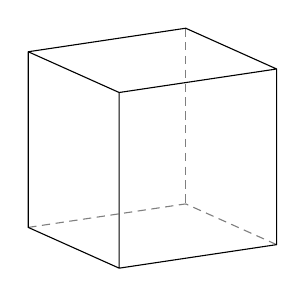
\begin{tikzpicture}[line join=round,x={(1cm, .1494cm)},y={(-.5774cm, .2588cm)},z={(0cm, 1.1154cm)}]
      \draw[every edge/.append style={densely dashed, opacity=.5}]
        (1,1,1) edge coordinate[at end] (obscured) (1,1,-1)
        -- (1,-1,1) -- (-1,-1,1) -- (-1,1,1) -- cycle
        (-1,1,-1) edge (obscured)
        -- (-1,1,1) -- (-1,-1,1) -- (-1,-1,-1) -- cycle
        (1,-1,-1) edge (obscured)
        -- (-1,-1,-1) -- (-1,-1,1) -- (1,-1,1) -- cycle;
    \end{tikzpicture}
  }
  \quad
  \subcaptionbox{A dodecahedron\label{fig:dodecahedron}}[0.3\textwidth]{
    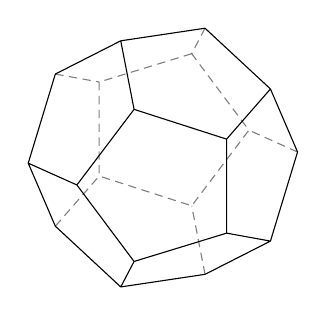
\begin{tikzpicture}[line join=round,x={(.8660cm, .1294cm)},y={(-.5cm, .2241cm)},z={(0cm, .9659cm)},declare function={phi()=(1 + sqrt(5)) / 2;}]
      \draw[densely dashed, opacity=.5]
        (1, 1, 1) -- (0, phi, 1/phi) -- (0, phi, -1/phi) -- (1, 1, -1) -- (phi, 1/phi, 0) -- cycle;

      \draw[every edge/.append style={densely dashed, opacity=.5}]
        (1/phi, 0, phi) edge (1, 1, 1)
        -- (1, -1, 1) -- (0, -phi, 1/phi) -- (-1, -1, 1) -- (-1/phi, 0, phi) -- cycle
        (-1, 1, 1) edge (0, phi, 1/phi)
        -- (-1/phi, 0, phi) -- (-1, -1, 1) -- (-phi, -1/phi, 0) -- (-phi, 1/phi, 0) -- cycle
        (-1, 1, -1) edge (0, phi, -1/phi)
        -- (-phi, 1/phi, 0) -- (-phi, -1/phi, 0) -- (-1, -1, -1) -- (-1/phi, 0, -phi) -- cycle
        (1/phi, 0, -phi) edge (1, 1, -1)
        -- (-1/phi, 0, -phi) -- (-1, -1, -1) -- (0, -phi, -1/phi) -- (1, -1, -1) -- cycle
        (phi, -1/phi, 0) edge (phi, 1/phi, 0)
        -- (1, -1, -1) -- (0, -phi, -1/phi) -- (0, -phi, 1/phi) -- (1, -1, 1) -- cycle;
    \end{tikzpicture}
  }
  \caption{
    Three shapes
  }
  \label{fig:shapes}
\end{figure}

For our shapes, the situation is no better.
Especially since the figure only shows the abstract essence of a tetrahedron, a cube, and a dodecahedron.
Were the figure to show any particular physical instances of these shapes, then at least we could have compared masses and lengths.
Luckily, abstract shapes can be measured too.
The number of corners, the number of edges, and the number of faces are a few of the metrics we can look at.
In all of these measures, a cube, Figure~\ref{fig:cube}, is larger than a tetrahedron, Figure~\ref{fig:tetrahedron}, and smaller than a dodecahedron, Figure~\ref{fig:dodecahedron}.
\begin{center}
  \begin{tabular}{r|p{2em}rp{1em}p{2em}rp{1em}p{2em}rp{1em}}
    &	\multicolumn{3}{c}{\emph{tetrahedron}}	& \multicolumn{3}{c}{\emph{cube}}	& \multicolumn{3}{c}{\emph{dodecahedron}} \\
    \hline
    \emph{corners}	&& $4$	&&& $8$	&&& $20$ \\
    \emph{edges}	&& $\phantom{0}6$	&&& $12$	&&& $30$	& \hspace{0pt} \\
    \emph{faces}	&& $4$	&&& $6$	&&& $12$
  \end{tabular}
\end{center}

None of these ways of measuring a shape, by the number of corners, edges, or faces, is clearly more fundamental than the others.
Besides, these ways of measuring are by no means all ways there are of measuring a shape.
Another metric looks at the number of edges that need to be traversed in order to get from one corner to another.
Let us consider this metric for the cube.
From each corner of the cube, only $3$~others are directly reachable.
Sometimes, traversing $2$ or even $3$~edges may be necessary.
Since we never need to go over more than $3$~edges, we say that the \emph{diameter} of a cube, in an abstract sense, is $3$~edges.
The diameter of a shape is another metric that may be used to measure a shape.

Yet another metric is defined by the minimum number of corners we need to mark so that every edge connects to a marked corner at one or both of its ends.
Such a collection of marked vertices is said to \emph{cover} the edges.
For a cube, it is possible to cover the edges using $4$~corners.
It is not possible to cover all the edges with fewer corners, thus $4$ is the minimum number of corners that is required to cover the edges.
Like our previous metrics, this minimum number of corners that is required to cover the edges of a shape may be used to measure a shape.

Which metric is the most relevant depends on what uses of our shape we are most interested in.
Our previous two metrics looked specifically at corners and edges.
In such cases, we are really only interested in the connection structure of a shape.
Its three-dimensional nature is of lesser interest and the cube may as well be represented as in Figure~\ref{fig:graphs:cube}.

\begin{figure}
  \centering
  \subcaptionbox{
    The abstract cube visualized as a graph.
    Corners of the cube are shown as dots and dots are connected by a line whenever the corners they represent are connected by an edge of the cube.
    \label{fig:graphs:cube}
  }[0.4\textwidth]{
    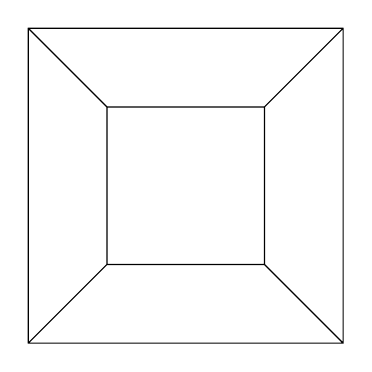
\begin{tikzpicture}[line join=round]
      \draw
        (0,0) -- (0,4) -- (1,3) -- (1,1) -- cycle
        (0,4) -- (4,4) -- (3,3) -- (1,3) -- cycle
        (4,4) -- (4,0) -- (3,1) -- (3,3) -- cycle
        (4,0) -- (0,0) -- (1,1) -- (3,1) -- cycle;
      \filldraw
        (0,0) circle[] (1,3) circle[]
        (0,4) circle[] (3,3) circle[]
        (4,4) circle[] (3,1) circle[]
        (4,0) circle[] (1,1) circle;
    \end{tikzpicture}
  }
  \qquad
  \subcaptionbox{
    The Wagner graph.
    Note that this graph can be obtained from the cube graph, Figure~\ref{fig:graphs:cube}, by exchanging two endpoints of two edges.
    \label{fig:graphs:wagner}
  }[0.4\textwidth]{
    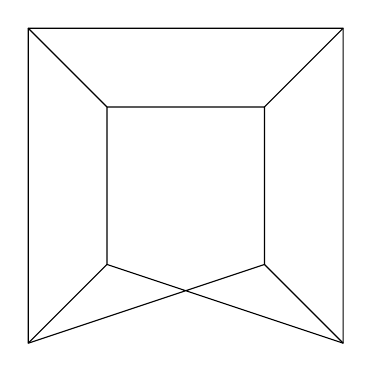
\begin{tikzpicture}[line join=round]
      \draw
        (0,0) -- (0,4) -- (4,4) -- (4,0) --
        (1,1) -- (1,3) -- (3,3) -- (3,1) -- cycle;
      \filldraw
        (0,0) circle[] -- (1,1) circle[]
        (0,4) circle[] -- (1,3) circle[]
        (4,4) circle[] -- (3,3) circle[]
        (4,0) circle -- (3,1) circle;
    \end{tikzpicture}
  }
  \caption{
    Structures of possibly connected objects can be represented as graphs.
    The dots in the above graphs represent the objects and are called \emph{vertices}.
    The lines connecting vertices are called \emph{edges}.
  }
\end{figure}

Note that for all simple graphs, there is a maximum to the number of edges as a function of the number of vertices.
Once all vertices in a graph are connected to each other, we cannot add any new edges to the graph.
On the other hand, if we allow for vertices that are not connected to any other vertex, then the number of vertices can be far greater than the number of edges.
In particular, there is then no maximum to the number of vertices as a function of the number of edges.
Moreover, there are only finitely many graphs with any given number of vertices, whereas there are infinitely many for any given number of edges.
For this reason, we may consider the number of vertices to be a more fundamental metric than the number of edges.
However, calling a graph with very many vertices but hardly any edges \enquote{large} may conflict with our intuitive notion of size.

Again, what graphs are large depends on what is meant by \enquote{large}.
In each context the appropriate notion of size may be different.
Roughly speaking, the size of an object relates to how difficult it is to work with.
The more extreme the dimensions or masses of objects are, the more inconvenient processing them will likely be.
This is true for the physical processing of physical objects, but also for processing abstract objects computationally.
It is the latter kind of processing that this thesis is concerned with.

Returning to graphs, some actions on graphs may conceivably be easier on graphs with a smaller diameter.
In the context of such actions, the diameter of a graph may be a good measure of the size of a graph.
Other contexts may favor graphs in which the edges can be covered by a smaller number of vertices.
A set of vertices that cover the edges of a graph is called a \emph{vertex cover}.
In contexts that favor small vertex covers, the minimum size of a vertex cover may be a good measure of the size of a graph.

As a demonstration of the possible disagreement between all these measures of the size of a graph, consider the graph in Figure~\ref{fig:graphs:wagner}.
This graph is known as the \emph{Wagner graph}.
Because it cannot be drawn without some edges crossing each other, there is no meaningful way we can assign a value to the number of faces of this graph.
Of course, there are also no corners in the way that our shapes had them, but the Wagner graph does have vertices, which can be counted just as well.
As far as the number of vertices or the number of edges are concerned, the Wagner graph, Figure~\ref{fig:graphs:wagner}, has the same size as the graph of the cube, Figure~\ref{fig:graphs:cube}.
\begin{center}
  \begin{tabular}{r|p{2em}rp{1em}p{2em}rp{1em}}
    &	\multicolumn{3}{c}{\emph{cube graph}}	& \multicolumn{3}{c}{\emph{Wagner graph}} \\
    \hline
    \emph{vertices}	&& $8$	&&& $8$ \\
    \emph{edges}	&& $12$	&&& $12$	& \hspace{0pt} \\
    \emph{diameter}	&& $3$	&&& $2$ \\
    \emph{vertex cover}	&& $4$	&&& $5$
  \end{tabular}
\end{center}
On our other two metrics, the graphs differ.
The Wagner graph has a smaller diameter than the cube graph.
By contrast, the minimum size of a vertex cover, listed simply as \enquote{\emph{vertex cover}} in the table above, is smaller for the cube graph.
Thus, we see that which of the two graphs is larger depends on the metric that is used and hence on the context in which we compare the two graphs.

\medbreak
In the next section of this chapter, Section~\ref{sec:history}, several more examples of the multifaceted nature of complexity are discussed more formally.
The remainder of this thesis then works towards a unified analysis of complexity that works for each of the forms of complexity we identify in Section~\ref{sec:history}.
Finally, in Section~\ref{sec:conclusion:size_of_a_cube}, we shall return briefly to measuring a cube, and summarize our findings.


\bigsection{Historical Encounters}
\label{sec:history}%

The word \emph{complexity} is used in various contexts and its meaning is not always made precise.
Still, it has often been observed that structural properties of data may influence the notion of complexity at hand.
In this thesis, we put forward a mathematical formalization of the notion of complexity, covering as many use cases as possible.
First, let us review some of the ways we may encounter complexity and what structural properties these many forms of complexity are involved with.
In relation to their notions of complexity, each of these structural properties points at a line of thinking that is essentially parameterized.
In Chapter~\ref{ch:parameterizations}, this parameterized nature is made explicit by rephrasing the corresponding results in a unified parameterized framework.
A historical overview of the theoretical side of parameterized reasoning can be found in Section~\ref{sec:conclusion:history}.

\subsection{Computability}
\label{sec:history:computability}%
Some sets are intrinsically undecidable.
For such sets, there is no effective procedure that is able to distinguish the members of the set from the nonmembers of the set.
This is a very extreme form of complexity:
We are unable to determine membership in undecidable sets uniformly not because we are perhaps not clever enough, but because it is fundamentally impossible.
Undecidable sets, however, are not all equally undecidable.
It is possible to organize many sets in a hierarchy of (un)decidability.
In fact, there are many ways to do so.

One hierarchy in which sets can be placed based on their decidability is the \defkey{arithmetical hierarchy}, due to \textcite{kleene1943recursive}.
This hierarchy consists of classes of sets that are defined inductively.
The classifications are denoted $\Sigma^0_n$ and $\Pi^0_n$, where $n$ is a natural number.
A set $S$ is in $\Sigma^0_{n+1}$ if there is a set $P$ in $\Pi^0_n$ such that we have
\begin{align*}
  S &= \{x \st \exists y\colon (x, y) \in P\}.
\intertext{
  Observe that the set $P$ is a set of pairs.
  Conversely, a set $P$ is in $\Pi^0_{n + 1}$ if there is a set of pairs $S$ in $\Sigma^0_n$ such that we have
}
  P &= \{x \st \forall y\colon (x, y) \in S\}.
\end{align*}
All that remains to define the arithmetical hierarchy is a definition of the base case, the classes $\Sigma^0_0$ and $\Pi^0_0$.
We follow \textcite{rogers1967theory,downey2010algorithmic} and set both classes equal to the class of decidable sets.
Originally, \citeauthor{kleene1943recursive} chose a smaller class, namely that of sets definable through \enquote{primitive recursive} predicates.
Yet another option is to take for $\Sigma^0_0$ and $\Pi^0_0$ the class of sets definable in first-order~logic with only bounded quantifiers~\parencite{odifreddi1992classical}.
We shall not go into details about these alternatives.
Whichever definition we adhere to, we end up with the same classes $\Sigma^0_n$ and $\Pi^0_n$, whenever $n$ is at least~$1$.
To wit, regardless of our choice for $\Sigma^0_0$ and $\Pi^0_0$, a set is in $\Sigma^0_1$ precisely when it is \emph{semidecidable} (also known as \emph{recursively enumerable})~\parencite{kleene1943recursive,odifreddi1992classical,rogers1967theory}.
Likewise, the complement of a semidecidable set is in $\Pi^0_1$, as $\exists$ and $\forall$ are dual to each other in the sense that, for every predicate~$Q$ we have
\begin{equation*}
  \lnot \exists x\colon Q(x) \:\iff\: \forall x\colon \lnot Q(x).
\end{equation*}
Indeed, a set $S$ is in $\Sigma^0_n$ precisely when there is a decidable set $A$ such that we have
\begin{equation}
\label{eq:arithmetical_hierarchy}
  S = \{x \st \exists y_1\colon \forall y_2\colon\exists y_3\colon \ldots\colon ((\cdots((x, y_1), y_2)\cdots, y_{n-1}), y_n) \in A\},
\end{equation}
and similarly for $\Pi^0_n$ when we exchange $\exists$ and $\forall$.
It follows that, in general, a set is in $\Sigma^0_n$ if its complement is in $\Pi^0_n$.
As, whenever $n$ is at least~$1$, the classes $\Sigma^0_n$ and $\Pi^0_n$ are unequal, neither is closed with respect to taking complements.
For convenience, we therefore define classes $\Delta^0_n$ as the intersection of $\Sigma^0_n$ and $\Pi^0_n$.
These classes \emph{are} closed with respect to taking complements.
Remark that sets in $\Delta^0_1$ are both semidecidable and have a semidecidable complement, and are therefore decidable.
Visually, the arithmetical hierarchy thus looks like depicted in Figure~\ref{fig:arithmetical_hierarchy}.
\begin{figure}
  \centering
  \begin{subfigure}{0.4\textwidth}
    \centering
    \begin{tikzpicture}
      \graph[layered layout, grow'=up, sibling distance=6em, edges={draw=none}, edge quotes={sloped, allow upside down}]{
        "$\Delta^0_0$" --["$=$"] {
          "$\Sigma^0_0$", "$\Pi^0_0$"
        } --["$=$"] "$\Delta^0_1$" ->["$\subset$"] {
          "$\Sigma^0_1$", "$\Pi^0_1$"
        } ->["$\subset$"] "$\Delta^0_2$" ->["$\subset$"] {
          "$\Sigma^0_2$", "$\Pi^0_2$"
        } ->["$\subset$"] "\vdots"
      };
    \end{tikzpicture}
    \caption{
      The arithmetical hierarchy
      \\\hspace{0pt}\\\hspace{0pt} % For alignment
    }
    \label{fig:arithmetical_hierarchy}
  \end{subfigure}
  \qquad
  \begin{subfigure}{0.4\textwidth}
    \centering
    \begin{tikzpicture}
      \graph[layered layout, grow'=up, sibling distance=6em, edges={draw=none}, edge quotes={sloped, allow upside down}]{
        "$\Delta^{-1}_1\mathrlap{\:= \Delta^0_1}$" ->["$\subset$"] {
          "$\mathllap{\Sigma^0_1 =\:}\Sigma^{-1}_1$", "$\Pi^{-1}_1\mathrlap{\:= \Pi^0_1}$"
        } ->["$\subset$"] "$\Delta^{-1}_2$" ->["$\subset$"] {
          "$\Sigma^{-1}_2$", "$\Pi^{-1}_2$"
        } ->["$\subset$"] "$\Delta^{-1}_3$" ->["$\subset$"] {
          "$\Sigma^{-1}_3$", "$\Pi^{-1}_3$"
        } ->["$\subset$"] "\vdots"
      };
    \end{tikzpicture}
    \caption{
      The difference hierarchy lies below the $\Delta^0_2$~level of the arithmetical hierarchy.
    }
    \label{fig:difference_hierarchy}
  \end{subfigure}
  \caption{
    The arithmetical hierarchy and the difference hierarchy are both infinite hierarchies of classes of sets.
  }
\end{figure}

Returning to undecidability as a form of complexity, the arithmetical hierarchy provides a means of analyzing complexity.
For sets that appear in one of the classes of the arithmetical hierarchy, say $\Delta^0_n$, we may call the level at which it occurs, $n$, \enquote{the complexity} of the set.
Thus, we can compare how undecidable certain sets are.
As demonstrated by~\eqref{eq:arithmetical_hierarchy}, this notion of complexity ties in with a more or less structural property of the set it applies to.
The number of quantifier alternations required for defining a set starting from a decidable set expresses its complexity.

At a conceptual level, one of the focal points of computability theory is the behavior of computations in the limit.
Computations that terminate eventually are said to \emph{converge}, and computations that never terminate are said to \emph{diverge}.
From this perspective, it is clear how the sets in $\Sigma^0_1$, the semidecidable sets, are slightly more complex than the decidable sets.
Decidable sets have decision procedures and those procedures converge on all inputs.
For semidecidable sets on the other hand, convergence of a procedure that tries to determine membership can only be guaranteed on the members of the set.
Ascending further in the arithmetical hierarchy, it becomes near-impossible to give characterizations of the sets in terms of convergence.
This is one reason to look for measures of complexity-beyond-decidability that increase complexity more gradually.
One such measure was introduced by \textcite{ershov1968hierarchyi} some 25 years after the introduction of the arithmetical hierarchy.
This measure also revolves around a hierarchy of classes of sets and is in that regard similar in spirit to the arithmetical hierarchy.
We have seen that the $\Sigma$ and $\Pi$ classes of the arithmetical hierarchy are not closed with respect to taking complements.
The starting point of \citeauthor{ershov1968hierarchyi}'s hierarchy was the observation that these classes are also not closed with respect to taking relative complements.
Given two sets $A$ and~$B$ in some class $\Sigma^0_n$, with $n$ at least~$1$, the set $A \setminus B$ need not be in $\Sigma^0_n$, and similarly for the classes $\Pi^0_n$.
However, when $A$ and $B$ are taken from~$\Sigma^0_n$, we may go about deciding whether a given~$x$ is in~$A \setminus B$ as follows.
\begin{codelisting}
\item
  We assume $x$ is neither in $A$ nor in $B$ and if our computations are interrupted and we are asked our best guess about $x$, we answer that it \emph{is not} in $A \setminus B$.
\item
  We try to find out whether $x$ is in $A$ by running a procedure that halts precisely on the members of $A$.
  If this procedure halts, we have learned that~$x$ is in~$A$.
  In case we are then asked our best guess about $x$, we answer that it \emph{is} in $A \setminus B$.
\item
  Having found that $x$ is in $A$, we try to find out whether $x$ is in $B$ by running a procedure that halts precisely on the members of $B$.
  If this procedure halts, we have learned that $x$ is also in $B$.
  In case we are later asked our best guess about $x$, we know the correct response and answer that it \emph{is not} in $A \setminus B$.
\end{codelisting}
Only in the final situation, we can answer a membership query with certainty.
Therefore, our procedure should be considered a kind of approximation of a decision procedure.
Observe that the procedure adjusts its knowledge about membership of $x$ in $A \setminus B$ at most twice.
Procedures that are not convergent in the classical sense, but are allowed to \enquote{change their mind} a finite number of times were first put forward by \textcite{putnam1965trial,gold1965limiting}.

The idea of \citeauthor{ershov1968hierarchyi} was to base a hierarchy on the number of times a decision procedure in the sense of \citeauthor{putnam1965trial} and \citeauthor{gold1965limiting} is allowed to change its mind.
The resulting hierarchy is known today as the \defkey{difference hierarchy}~\parencite{downey2010algorithmic,soare2016turing}.
The classes of the difference hierarchy are denoted $\Sigma^{-1}_n$ and $\Pi^{-1}_n$.
For sets $A$ and~$B$, let $A \symdiff B$ denote the \defkey{symmetric difference} $(A \setminus B) \cup (B \setminus A)$.
A set~$S$ is in~$\Sigma^{-1}_n$ if there are sets $A_1, A_2, A_3, \ldots, A_n$ in $\Sigma^0_1$ such that we have
\begin{equation}
\label{eq:difference_hierarchy}
  S = A_1 \symdiff A_2 \symdiff A_3 \symdiff \cdots \symdiff A_n.
\end{equation}
Like in the arithmetical hierarchy, a set~$P$ is in~$\Pi^{-1}_n$ if its complement, $P^\complement$, is in~$\Sigma^{-1}_n$.
Note that when $n$ is odd, we have
\begin{equation*}
  (A_1 \symdiff A_2 \symdiff A_3 \symdiff \cdots \symdiff A_n)^\complement = A_1^\complement \symdiff A_2^\complement \symdiff A_3^\complement \symdiff \cdots \symdiff A_n^\complement.
\end{equation*}
Therefore, for odd $n$, a set~$P$ is in~$\Pi^{-1}_n$ if there are sets $A_1, A_2, A_3, \ldots, A_n$ in~$\Pi^0_1$ such that we have
\begin{equation*}
  P = A_1 \symdiff A_2 \symdiff A_3 \symdiff \cdots \symdiff A_n.
\end{equation*}
These definitions are equivalent to the original characterization by \textcite{ershov1968hierarchyi} that was stated in terms of unions of disjoint relative complements.
The equivalence follows from elementary identities.
The resulting hierarchy, including the levels~$\Delta^{-1}_n$ that are the intersection of $\Sigma^{-1}_n$ and $\Pi^{-1}_n$, is depicted in Figure~\ref{fig:difference_hierarchy}.

Because the $\Delta^0_2$ class is closed under taking unions, intersections, and complements, it is also closed under taking symmetric differences.
Moreover, it includes both $\Sigma^0_1$ and $\Pi^0_1$, thus for all natural numbers $n$, the classes $\Sigma^{-1}_n$, $\Pi^{-1}_n$, and $\Delta^{-1}_n$ of the difference hierarchy are included in $\Delta^0_2$.
Consequently, the difference hierarchy is only relevant for sets that are not too complicated according to the arithmetical hierarchy.
Still, its core ideas make the ensuing notion of complexity an interesting measure of undecidability.
As we have seen, the number of semidecidable sets needed to write a set like in~\eqref{eq:difference_hierarchy} relates to a generalized form of convergence of computation.

\subsection{Computational Tractability}
\label{sec:history:tractability}%
In computational complexity theory, a set is deemed complex if it is intractable.
Here, tractability is customarily taken with respect to the running-time behavior of decision procedures.
While we can measure the time a decision procedure takes on a specific input, we are primarily interested in how this time compares to other, unknown, inputs.
The running time of a decision procedure is therefore traditionally expressed as a function of the size of its input.
As we saw in Section~\ref{sec:size_of_a_cube}, the notion of input size is heavily reliant on the choice of an encoding scheme for inputs.
No computable encoding scheme reflects all possible structural aspects an input may have.
This is especially visible in contexts that offer some \enquote{standard} encoding.
For instance, in graph theory~\parencite{diestel2017graph}, graphs are often thought of as encoded by an adjacency matrix.
In that case, the size of a graph is determined by the number of its vertices.
However, certain structural properties other than the number of vertices may be exploitable by a decision procedure for a set of graphs.
Regarding sets that are intractable because the running time of a decision procedure is at least exponential as a function of the input size, \citeauthor{garey1979computers} remark the following.
\blockcquote[Section~4.3]{garey1979computers}{
  \textelp{} there are a variety of ways in which the time complexity of an algorithm can be \enquote{exponential,} some of which might be preferable to others.
  This is especially evident when, as is customary in practice, we consider time complexity expressed in terms of natural problem parameters instead of the artificially constructed \enquote{input length.}
}
When restricting to inputs on which such \emph{natural parameters} assume small values, a set that is initially intractable may indeed become tractable.
As inputs with low parameter values may be abundant, it may be that large subsets of the input space are easy to digest for some decision procedure.
In addition, \citeauthor{garey1979computers} note that inputs encountered in practice may tend to have low parameter values:
\enquote{\textelp{} in practice it is often the subproblem, rather than the general problem, that we are called upon to solve.}

\begin{example}
\label{ex:type_inference}%
  The standard compilers for the Rust programming language and the Haskell programming language are able to infer data types of variables and functions.
  The algorithm they use for this has a worst-case running-time that scales exponential as a function of the length of its input.
  However, such exponential running times are experienced very rarely in practice~\parencite{kanellakis1989polymorphic}.
  Thus, some property of the expressions that this algorithm operates on behaves in a special way for inputs that are encountered in practice.
  Indeed, the origin of the exponential running time of the algorithm can be traced back to the nesting depth of a certain pattern in the expressions.
  In practice, this nesting depth is almost always low.
\end{example}

\begin{example}
\label{ex:clique}%
  We can model a social network by a graph, representing persons by vertices and connecting two vertices when the persons they represent know each other.
  Given a graph that models mutual acquaintance, we may ask how large a subset of people there exists that all know each other~\parencite[a \emph{clique}, see][]{diestel2017graph}.
  This is formalized by the set
  \begin{align*}
    \defkeyat{Clique@\pr{Clique}}{\pr{Clique}} \deq \{(G, l) \st &\text{there is a set of at least $l$ vertices of the graph~$G$ in which} \\
    	&\text{each pair of vertices is connected by an edge}\},
  \end{align*}

  Let $G$ be a graph with $n$ vertices and let $l$ be at most $n$.
  The number of possible subsets of the vertices of $G$ that are of size $l$ cannot be bounded by a polynomial of $n$ alone.
  In fact, when $l$ is, say, $\frac{n}{2}$, the number of subsets is exponential as a function of $n$.
  It is widely believed that there are no decision procedures for \pr{Clique} that have a subexponential running time.
  Nonetheless, given a subset of vertices of $G$, we can check whether its members are pairwise connected within a polynomial running time.

  However, this analysis disregards some practicalities that result from the situation we are modeling.
  It is rare to come across a person with very many mutual acquaintances.
  Therefore, it is safe to assume that in any graph we that models a social network, almost no vertex is connected to more than, say, $20$ others.
  As a consequence, we find that in any graph encountered in practice, a set of pairwise connected vertices, a \emph{clique}, can contain at most $21$ elements.
  This means that the number of subsets of vertices that needs to be checked is less than $n^{21}$, which, as \citeauthor{garey1979computers} observe~\parencite[Section~4.1]{garey1979computers}, is polynomial in~$n$.
  While this already brings the running time down to polynomial, we shall see in Section~\ref{sec:parameterized_complexity_theory} that a far more efficient decision procedure is not hard to come by.
\end{example}

The takeaway is that computational complexity is preferably measured by parameters of the input instead of by the input length alone.
Somehow, we need to decide which parameters to take into account.
Different decision procedures may favor different parameters.
Note, though, that it is possible to combine the benefits that different parameters may provide through aggregating multiple decision procedures.

\begin{example}
  \indexkey{Clique@\pr{Clique}}%
  One way to decide membership in \pr{Clique} is by generating an exhaustive list of candidate sets of vertices and checking whether any is a clique of the desired size.
  Suppose we want to decide whether a given graph $G$ has a clique of $l$ elements.
  The simplest implementation of the aforementioned design pattern starts out by generating all possible sets of $l$ vertices of $G$.
  However, other approaches are possible too.

  Suppose $l$ is even and we have a clique $(v_1, v_2, v_3, \ldots, v_l)$.
  Because these vertices form a clique there is, for $i \le \frac{l}{2}$, an edge connecting $v_i$ to $v_{i + \frac{l}{2}}$ in $G$.
  Thus an alternative way to generate candidate sets of vertices is via all possible sets of $\frac{l}{2}$ edges, by taking the endpoints of the selected edges.
  Any clique of size $l$ is guaranteed to be generated this way.

  We can compare these two approaches by counting the number of candidate sets they consider.
  Let $n$ be the number of vertices in~$G$ and $m$ the number of edges in~$G$.
  There are $\binom{n}{l}$ sets of $l$ vertices and $\binom{m}{l / 2}$ sets of $\frac{l}{2}$ edges.
  When either of these numbers is much smaller than the other, we expect the corresponding decision procedure to run much faster than the other.
  Thus, it pays to construct an aggregate decision procedure.
  This decision procedure would first compute both numbers and then run the decision procedure that is expected to be the fastest.

  The computational complexity of the vertex-centric decision procedure is best expressed as a function of the parameters $n$ and $l$.
  On the other hand, the complexity of the edge-centric decision procedure is best expressed as a function of the parameters $m$ and $l$.
  Our aggregate decision procedure demonstrates that it pays off to take into account multiple parameters.
  By taking into account more parameters, we get a more detailed insight into the computational complexity of a set such as \pr{Clique}.
  For some instances of \pr{Clique}, the running-time bound available in terms of $n$ and $l$ is better than that in terms of $m$ and $l$ and vice versa.
\end{example}

The algorithm we presented for our aggregate decision procedure for \pr{Clique} in the example above combines two other algorithms.
Such algorithms are known as \emph{hybrid algorithms}~\parencite{malek1994hybrid}.
They offer a best-of-both-worlds alternative in situations where we have two algorithms without one being better than the other.
From a parameterized point of view, hybrid algorithms combine the information of multiple input parameters and as such show how these parameters can interact.
This is relevant not only when we use parameters to measure computational complexity, but also in the design of ever-faster polynomial-time algorithms.

\begin{example}
  \indexkey{example!sorting algorithms}%
  As a showcase of hybrid algorithms that do not face computational intractability, we shall take a look at sorting algorithms.
  Even naive sorting algorithms, such as repeatedly finding the least value, manage to have a running time bounded by a polynomial of the length of the input list.
  Because sorting is such a common operation in algorithmics, extensive research has been put into the development of fast sorting algorithms.

  The quicksort algorithm \parencite{cormen2009introduction} makes a number of comparisons that is at most quadratic as a function of the length, $n$, of the input list.
  However, worst-case inputs are very rare and on average the algorithm needs roughly $n \log n$ comparisons.
  With a number of comparisons in the order of $n \log n$ in the worst case, the heapsort algorithm \parencite{cormen2009introduction} appears at least as good as quicksort.
  Nevertheless, it has a higher overhead and in practice it is often outperformed by quicksort.
  By combining both algorithms, we can construct a sorting algorithm that is about as fast as quicksort, yet has a worst-case running time in the order of $n \log n$.
  This hybrid algorithm is known as \emph{introsort} \parencite{musser1997introspective} and is used by some prominent implementations of the \Cpp{} standard library.

  The way introsort chooses between its constituent algorithms, quicksort and heapsort, is not as up-front as it was in our hybrid decision procedure for \pr{Clique}.
  This matters when we want to identify parameters that express structure favored by either of the constituent algorithms.
  Instead of handing over the input to either quicksort or heapsort, the hybrid introsort hooks into the divide-and-conquer nature of quicksort.
  The core of the quicksort algorithm is that it splits its input list into a list of low values and a list of high values.
  These sublists can be sorted independently and for that, quicksort recursively invokes itself.
  Because the splitting stage requires some $n$ comparisons for a list of $n$ elements, we do not want the recursion depth to exceed a constant multiple of $\log n$.
  In the worst case, however, quicksort reaches a recursion depth of $n$.
  To mitigate this worst case behavior, introsort uses heapsort to sort the sublists when the recursion depth gets too high, say higher than $2 \log n$.
  Thus, we have found that the recursion depth reached by quicksort functions as a parameter of the input list.
  This parameter may appear somewhat unnatural and its specific value for a given list depends on the implementation of quicksort.
  For all implementations, however, input lists that get high parameter values can be constructed~\parencite{mcilroy1999killer}.

  For short lists, insertion~sort \parencite{cormen2009introduction} is faster still than quicksort and heapsort.
  However, it makes a quadratic number of comparisons in the average case.
  Therefore it is suboptimal for all inputs of a length exceeding some platform-dependent constant.
  Many implementations of introsort use insertion~sort when the input list is short.
  Here, the parameter at play is evident.
  It is the length of the input list.

  The architecture of introsort follows quicksort and only for the base case of the recursion it deviates from that.
  In this way, introsort is based on an algorithm that has a bad worst-case running time, but is  fast in practice.
  Another hybrid sorting algorithm, timsort \parencite{peters:timsort}, takes the opposite approach.
  This algorithm was developed for the Python programming language and is also used in the Java virtual machine and in the standard library of the Rust programming language.
  It is adapted from mergesort \parencite{cormen2009introduction}, which has a good worst-case running time, but fails to exploit patterns encountered in practice.
  Like quicksort, mergesort is a divide-and-conquer algorithm.
  Where introsort followed quicksort top-down and resorted to heapsort at high recursion depths, timsort follows a bottom-up implementation of mergesort.
  It uses insertion~sort on small chunks of the input to quickly prepare a base case that is as accommodating to mergesort as possible.
  Using insertion~sort for the base case is efficient, because insertion~sort is fast on short lists.
  The base case is prepared in such a way that the use of locally sorted parts of the input list is maximized.
  This makes timsort an \emph{adaptive} sorting algorithm.
  A proper analysis of timsort is therefore not possible on the basis of only the length of the input list as a parameter.
  In addition, it requires a parameter related to the locality of the disorder in the input list.
\end{example}

Note that a detailed analysis of the computational complexity of an algorithm may expose many parameters that influence the running time of the algorithm.
These parameters need not be independent of one another, and their interactions need not be straightforward.
Parameterized computational complexity theorists are tasked with gaining insight in these interactions.

\subsection{Algorithmic Complexity}
\label{sec:history:algorithmic}%
Complexity, in whatever incarnation, can often be traced back to a lack of structure.
Objects that are evidently highly structured are easy to analyze and an unlikely cause of complexity.
But what makes an object structured?
One answer could be \enquote{if it has many properties}, but this simply makes us wonder what counts as a property of an object.
Certainly, we want the properties of an object to tell us something about the object.
In other words, it must be special for an object to have a given property.
We mean this in a technical sense and assert that structural properties help in giving short descriptions of objects.

\begin{example}
  Consider graphs on $8$~vertices.
  There are
  \begin{align*}
    2^{\binom{8}{2}} &= \num{268435456}
  \intertext{
    such graphs.
    However, if we know that a particular graph has $9$~edges, we are left with only
  }
    \binom{\binom{8}{2}}{9} &= \phantom{00}\num{6906900}
  \end{align*}
  options.
  Because this is a substantial reduction, we can give a succinct description of a graph with $8$~vertices and $9$~edges by first giving its number of edges.

  The critical observer will have noticed that we have assumed a number of vertices that was fixed and known.
  Indeed, having $8$~vertices is in itself already a structural property of a graph.
  Without knowing the number of vertices in a graph that is being described to us, we have an infinite number of candidates to choose from.
\end{example}

Often, we can identify a value inside a structural property that can be generalized over.
The property can then be seen as an instantiation of an underlying property schema.
This is most apparent when the structural property has an element of counting in it, such as is the case with our \enquote{has $9$~edges} property in the example above.
\begin{example}[continued]
\label{ex:edges}%
  Replacing the value~$9$ in the property \enquote{has $9$~edges} by the variable $e$, we obtain the property schema \enquote{has $e$~edges}.
\end{example}

Seldomly is it necessary to make a distinction between properties and property schemata.
However, it is useful here because it clarifies the relation between parameters, as encountered earlier, and properties.
Technically, parameters correspond to property schemata.

When describing objects, it is necessary to settle, beforehand, what counts as a reasonable description method.
Were we to allow all possible mappings of objects to strings, we run into paradoxes like the Berry paradox \parencite[see][]{li2008introduction}.
This paradox shows that if any mapping goes, any object could be described in arbitrarily few bits.
The argument is simple: if it would not be so, then we could take the first among the counterexamples and map an arbitrarily short description to it, violating it being a counterexample.
Therefore, we prefer to work with computable total functions as description methods.
Each description method is thus assigned a length according to a specification of the performed computation.
Doing so, we get, for each object, a lower bound on the sum of the length of the description method used and the length of a description of the object.
This bound is the Kolmogorov complexity of the object.
Indeed, any structure in an object is picked up by its Kolmogorov complexity.
This urges an investigation of the use of the Kolmogorov complexity as a parameter, as the property schema \enquote{has a Kolmogorov complexity of at most~$c$}.
However, the Kolmogorov complexity is not itself a computable function, so such an investigation would take us outside the realm of reasonable description methods.

Next to thinking of Kolmogorov complexity as a parameter itself, we may think of Kolmogorov complexity as emerging from an assembly of all parameters.
A property can be thought of as a set of objects, namely the objects that have that property.
Any object that has a property can then be specified by its index in this set.
This interpretation of properties was already present in our example with the \enquote{has $9$~edges} property.
From this interpretation, it is a small step up to a kind of meta-property, the property schema \enquote{has property~$q$}.
As before, we want our description method to adhere to a form of computability.
We therefore assume that a property~$q$ is specified in the form of a decision procedure for the set of objects that have property~$q$.
These decision procedures are computable total functions.
However, there is no decision procedure that recognizes precisely the computable total functions.
Therefore, whether any given $q$ represents a reasonable property in the sense that it corresponds to a computable total function cannot be decided uniformly.

Alternatively, the undecidability of our meta-property can be deduced from the observation that this property schema too relates to Kolmogorov complexity.
An object represented by some~$x$ is the only object that has the property \enquote{equals~$x$}.
It should be clear that the shortest specification of this property has a length equal to the Kolmogorov complexity of~$x$.
Moreover, the index of~$x$ in the set of objects that adhere to this property is~$1$.
Hence, the length of a description according to this property added to the length of this property is about equal to the Kolmogorov complexity of~$x$.
At the same time, no two-part code can give description of~$x$ of a length shorter than the Kolmogorov complexity of~$x$.
Hence our parameter, the property schema \enquote{has property~$q$}, is also closely related to Kolmogorov complexity.

The analysis of Kolmogorov complexity as emerging from an assembly of all parameters has brought us one abstraction level up in the analysis of parameters.
Instead of working with individual parameters, we now work with sets of, not necessarily related, parameters.
When a certain set of parameters has our interest, we may ask how good of an approximation to the Kolmogorov complexity the ensuing two-part code is.
Of course, we should also ask whether or not the set of parameters is in any way decidable.
Taking the abstraction even further, we may look at ways to define sets of parameters.
For instance, given a computationally hard decision problem, we may consider those parameters that are responsible for the computational hardness.
This then leads to a notion of complexity in its own right.
If two decision problems lead to the same set of parameters, we could say that the computational complexity of the two problems has the same origins.
While exciting, this notion of equivalent computational complexity through identical sets of parameters has not seen much attention yet.

\subsection{Algorithmic Statistics}
A picture is worth a thousand words, or, in more convoluted terms, not all media are equal when it comes to the presentation of information.
This sets information apart from computability, which remains unchanged on a large class of machine models.
In the landmark paper in which he introduced his machine model, \citeauthor{turing1937computable} wrote the following about the use of one dimension or two dimensions in \emph{computation}.
\blockcquote{turing1937computable}{
  In elementary arithmetic the two-dimensional character of the paper is sometimes used.
  But such a use is always avoidable, and I think that it will be agreed that the two-dimensional character of paper is no essential of computation.
  I assume then that the computation is carried out on one-dimensional paper, i.e.~on a tape divided into squares.
}
A similar statement is arguably not true of \emph{information}.
In the presentation of information, using one dimension or two dimensions makes a difference.

\begin{example}
  Consider the following one-dimensional sequence of squares, some of which are filled.
  \begin{center}
    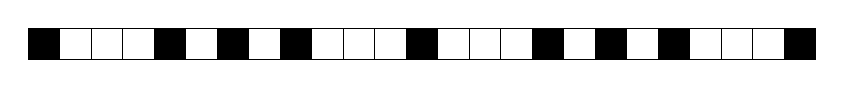
\begin{tikzpicture}
      \draw[step=4mm] (0,0) grid (10,.4);
      \fill%[pattern=north east lines]
        (0,0)   rectangle (.4,.4)  (1.6,0) rectangle (2,.4)
        (2.4,0) rectangle (2.8,.4) (3.2,0) rectangle (3.6,.4)
        (4.8,0) rectangle (5.2,.4)
        (6.4,0) rectangle (6.8,.4) (7.2,0) rectangle (7.6,.4)
        (8,0)   rectangle (8.4,.4) (9.6,0) rectangle (10,.4);
    \end{tikzpicture}
  \end{center}
  We can spot pretty quickly that this sequence is a palindrome.
  However, a far stronger geometrical relationship between the filled squares becomes evident when we present the same sequence as a two-dimensional grid.
  \begin{center}
    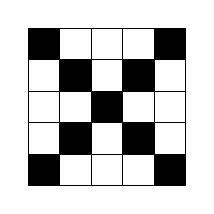
\begin{tikzpicture}
      \draw[step=4mm] (0,0) grid (2,2);
      \fill%[pattern=north east lines]
        (0,0)    rectangle (.4,.4)
                 rectangle (.8,.8)
                 rectangle (1.2,1.2)
                 rectangle (1.6,1.6)
                 rectangle (2,2)
        (2,0)    rectangle (1.6,.4)
                 rectangle (1.2,.8)
        (.8,1.2) rectangle (.4,1.6)
                 rectangle (0,2);
    \end{tikzpicture}
  \end{center}
  This goes to show that certain modes of presentation are preferred for certain patterns.
  Not all information is equally accessible in all modes of presentation.
\end{example}

For a more thorough treatment of informativeness, we need a formal description of what we mean by information.
Typically, we link information to \emph{entropy}~\parencite{cover2006elements}, thus bringing statistics on board the study of informativeness.
Information, then, relates to a property of a data source that expresses how unpredictable the data source is.
In other words, information is what breaks the mold, as it defies our expectation.
We remark that there is more to information than entropy alone, but refer the interested reader to the philosophical overview by~\textcite{adriaans2008philosophy}.

Different kinds of data come with different expectations.
Some patters are more clearly presented in certain modes of presentation, and conversely some modes of presentation make us expect certain patterns.
A musical idea, for example, is hard to convey in a painting, yet may be precisely what an audience member in a concert is listening for.
The medium is thus part of the message and information is context-dependent.

\begin{example}
\label{ex:pin}%
  \indexkey{example!distribution of PINs}%
  \pgfmathsetmacro{\numpasswords}{14830591}%
  Let us take a look at the distribution of passwords that are made up of four digits.
  Four-digit passwords are the de~facto norm for a personal identification number, a PIN.
  A naive analysis would be that when we have no information about someone's PIN and we have to guess it, we stand a one in ten~thousand chance of being correct.
  As we shall see, this is far from the truth when the PIN was chosen freely by its owner.

  To estimate the distribution of PINs in use, we filter a collection of over half a billion passwords for four-digit passwords.
  The collection is made up of passwords obtained in data breaches and was put together by \textcite{hunt2018have}.
  This tactic was first employed by \textcite{berry2012pin} and our approach here is much the same as his.
  In the database we use, \num{\numpasswords} uses of a four-digit password are recorded.
  Based on the relative frequency of each PIN, we quickly find that they are not distributed uniformly.
  As can be seen in Figure~\ref{fig:pinprobability}, the bulk of the distribution of PINs can be approximated by a straight line in a log--log plot.
  Therefore, our PINs are an example of a dataset that adheres to Zipf's law.
  This empirical law states that the frequency of a word in a corpus of natural language is inversely proportional to its rank.
  Outside natural language, distributions of this kind have been observed in many real-world data encountered in the physical and social sciences~\parencite{newman2005power}.
  \begin{figure}
    \centering
    \begin{tikzpicture}
      \begin{loglogaxis}[
        width=10cm,
        height=15cm, % Will be reduced automatically
        axis equal image=true,
        clip mode=individual,
        xlabel={rank},
        ylabel={empirical probability},
      ]
        \addplot [
          only marks,
          mark=+,
          scatter,
          scatter/use mapped color={draw=mapped color},
          point meta={max(1, min(10000, (55*\thisrowno{2}/\numpasswords)^(-1/0.7)))},
        ] table [
          header=false,
          x index=3,
          y expr={\thisrowno{2}/\numpasswords},
        ] {pwned.dat};
        \addplot [
          samples at={1, 10000},
        ] {x^(-0.7) / 55};
      \end{loglogaxis}
    \end{tikzpicture}
    \caption{
      A log--log plot of the empirical probability of PINs by rank, in decreasing order of likelihood.
      Except for one outlier on the top-end, the PIN~\code{1234}, and a thin tail of less than 5\% of the PINs, the distribution can be approximated by a power law.
      Points are colored in accordance with their rank as approximated by the fitted power law.
      Because the horizontal axis is logarithmic, the colormap appears distorted.
    }
    \label{fig:pinprobability}
  \end{figure}

  Having found that PINs are not distributed uniformly, we wonder what can be said about the specifics of their distribution.
  In Figure~\ref{fig:pinprobability}, we cannot see which PINs correspond to which data points.
  Therefore, we turn to a different plot, depicting the rank of all PINs as estimated by our approximation of the empirical probability distribution, Figure~\ref{fig:pinheatmap}.
  \begin{figure}
    \centering
    \begin{tikzpicture}
      \begin{axis}[
        x=1mm, y=1mm,
        enlargelimits=false,
        tick align=outside,
        xtick={10, 20, ..., 90},
        extra x ticks={0},
        extra x tick labels={$00$},
        ytick={10, 20, ..., 90},
        extra y ticks={0},
        extra y tick labels={$00$},
      ]
        \addplot [
          matrix plot*,
          point meta={max(1, min(10000, (55*\thisrowno{2}/\numpasswords)^(-1/0.7)))},
          mesh/cols=100,
        ] table [
          header=false,
        ] {pwned.dat};
      \end{axis}
    \end{tikzpicture}
    \caption{
      A heatmap of PINs, inspired by a similar heatmap created by \textcite{berry2012pin}.
      The first two digits of the PIN determine its horizontal position, while the last two digits determine the vertical position.
      This way, the PIN~\code{0099} ends up at the top-left corner and the PIN~\code{9900} ends up at the bottom-right corner.
      The colors are based on the clamped power law fitted on the bulk of the PINs in Figure~\ref{fig:pinprobability}.
      Darker colors represent more frequent occurrence of a PIN in the database.
      As witnessed by the area of light-colored PINs on the left side of the plot, many PINs in the tail of the distribution start with a~\code{0}.
    }
    \label{fig:pinheatmap}
  \end{figure}

  In Figure~\ref{fig:pinheatmap}, we can recognize many categories of PINs that occur frequently.
  Some of these categories are purely syntactical.
  The prominent diagonal line, for instance, represents PINs of the form \code{xyxy}.
  Algorithmic complexity theory is well-suited to deal with such patterns.
  We may therefore expect the universal distribution~\parencite{li2008introduction}, though uncomputable, to be a good model for the distribution of PINs.
  For this to be true, all structure in Figure~\ref{fig:pinheatmap} must be essentially syntactical.
  However, there is also a strong vertical line of PINs of the form \code{19xy}, continuing shortly into the \code{20xy} pattern.
  The prevalence of such PINs can easily be explained as people choosing a year as they PIN and most emotionally meaningful years being in the recent past.
  This explanation is not a syntactical one.
  Of course, a model for algorithmic complexity can include this contextual information at the cost of only an additive constant.
  With little more modeling of context, also the frequent occurrence of PINs formatted as dates, MMDD or DDMM, can be covered.
  The lengths of the months generate a distinct and recognizable pattern in our heatmap.
  Yet, we claim that the additive constant relative to a standard abstract definition of Turing machines will quickly become significant.
  Relative to the limited complexity of four-digit PINs, the cost of modeling all contexts that influence the choice of a PIN is huge.
  Some properties of the plot in Figure~\ref{fig:pinheatmap} can easily be explained culturally, but lack any numerical meaning.
  For instance, the PIN~\code{5683} occurs particularly often, which can be explained by its meaning as a phoneword.
  A phoneword is a word spelled on a traditional phone keypad using ITU~E.161 assigned letters.
  The letters of the word \enquote{Love} are assigned the digits~\code{5683}, respectively.
  It is thus not reasonable to expect the distribution of PINs to approximate the universal distribution in any way.
  We are better off identifying as many meaningful categories of PINs and build our model of PINs from there.
\end{example}

We can try to model a multitude of contexts so that we can deal with the information in each of them.
In doing so, however, we should control the amount of detail with which we describe our models.
Surely, we do not want a tailor-made model for every conceivable arrangement of data.
In such a setting, every data sample would have a context in which the sample contains no information.
This is known as \emph{overfitting}~\parencite{grunwald2007minimum}.
\emph{Algorithmic statistics} addresses overfitting by taking into account the complexity of a description of a model.
Interestingly, there are data sets for which no \emph{simple} model is a decent fit.
There are complex models in relation to which these data sets contain disproportionately little information.
In relation to any simple model, the information in these data sets is considerably higher.
From this observation, it follows that the minimum model complexity required to achieve a decent fit is a nontrivial property of a data set.
Thus, a parameterized analysis of data sets, where the parameter is this minimum model complexity, emerges.

In traditional algorithmic statistics, Kolmogorov complexity is used in the assignment of complexity to models.
By doing so, it is possible to include practically all effective models in the analysis of informativeness.
As a result, the central probability distribution of interest in traditional algorithmic statistics is the universal distribution.
We have seen in Example~\ref{ex:pin} that the universal distribution is not always the best for a particular domain.
Fortunately, it is possible to employ the methods of algorithmic statistics in a setting where we restrict our attention to a specific collection of models.

\subsection{Computational Redundancy}
At the end of Moore's~law, advances in computer engineering are no longer visible as more powerful computation, but instead as more ubiquitous computation.
With this shift, the choice of \emph{where} to perform computation, along with \emph{when} to perform \emph{how much} of it, becomes increasingly influential.

\begin{example}
  There are many ways to store digital information, ranging from dynamic random access memory to magnetic tape and optical discs.
  Each storage medium has its own strengths and weaknesses.
  Storage can be classified according to different metrics, such as cost per bit, availability, or access speed.
  Typically, embedded volatile memory is fast, but expensive, whereas archived non-volatile memory is cheap, but slow.
  It is commonplace for applications to make use of different types of memory for different types of data, depending on the anticipated use.
  For a large database, cost is a primary concern, while the cache of a dynamic algorithm is best served by memory that is as fast as possible.
  In practice, this means the database may be stored on an off-site storage server, while the dynamic algorithm makes use of the CPU~cache.

  For computation, similar considerations can be made.
  Computing on a mobile device may provide very low latency, yet faces bottlenecks in terms of speed and energy consumption.
  The alternative would be to move computation to an external computer.
  This architecture, treating computation as a service, is nowadays known as cloud computing.
  Offloading computation becomes interesting when a computational workload is more demanding than the locally available computational power.
  One possibility is that the workload is inherently heavy, as is the case for rendering computer-generated imagery.
  Another possibility is that the local computational power is limited, as is the case when cross-compilation for embedded devices is used.
\end{example}

There is an interplay between the location where data is stored and the location where computation is performed.
The two are best kept close together, and modern databases implement increasingly rich query languages \parencite[see also][]{agarwal2015succinct}.
An extreme example is provided by the {Apache} {Hadoop} Distributed File System.
Its manual phrases it as follows.
\blockcquote{borthakur:hdfs}{
  A computation requested by an application is much more efficient if it is executed near the data it operates on.
  This is especially true when the size of the data set is huge.
  This minimizes network congestion and increases the overall throughput of the system.
  The assumption is that it is often better to migrate the computation closer to where the data is located rather than moving the data to where the application is running.
}

Note that a server may be highly capable as a data storage facility, yet be unimpressive in its computational abilities.
The converse is possible as well.
In both cases, we may still want to minimize the cost of communication with the server.
For this, it becomes necessary to recognize redundancy in our computational task and leave it out of transmission.
\begin{example}
  Suppose we want to render many frames of an animation on a so-called \enquote{render farm}.
  This requires the transmission of a description of the computational task for each frame.
  The animation may, however, contain duplicate frames.
  It is worthwhile to preprocess our data and remove all duplicate frames before invoking the render farm.
  This preprocessing operation does not require much computational effort from our side, yet it might reduce the amount of data transmitted substantially.

  Conversely, if we want to perform a computation on data stored in an external database, it may be beneficial for the database to preprocess the data.
  To accomplish this, we not only send the database a request for certain data, but also a description of the operation we want to perform on it.
  The database may then spend a limited amount of time analyzing the data in terms of computational redundancy, and omit any identified redundancy from its reply.
  Again, with the proper time limit, this requires minimal computational effort from the database, yet may reduce the total amount of communication taking place.
\end{example}

When the computational context of data is known already when the data is recorded, it may be beneficial to perform the preprocessing step early on.
Doing so may save the database some storage capacity, or at least bring the storage requirement more in line with the computational complexity of the data.
As our database may not have great computational power, it is important that we limit preprocessing to computation that can be performed quickly.

With our examples so far, we have thought of machines connected via a network as atomic units of computation.
However, also within a computer, there are many independent units capable of computing.
These are the device controllers and other management systems that all run their own firmware.
Traditionally, such systems are extremely limited in their computational power.
This power has, however, been increasing steadily, and the potential of these devices to run application-level code has long been recognized \parencite[for example][]{riedel1998active}.
We have seen that preprocessing can reduce traffic on the network connecting computers.
Similarly, preprocessing can reduce traffic on the system bus connecting components inside a computer.

For certain computational tasks, a useful separation into a computationally redundant and a computationally hard part may be possible.
For others, it may be impossible to find such a clear-cut separation that is of any practical value.
This does not mean that we cannot benefit from remote computational powers.
Sometimes, a computational task is really a serialization of multiple subtasks, the specifics of each subtask depending on the outcome of the previous one.
With such a compound task, we may be able to identify computational redundancy in each subtask as we get to it.
In that case, making use of preprocessing for each of the subtasks requires a form of communication between the computational parties.
The party holding the data performs the preprocessing and communicates to the computationally powerful party the data relevant to the current subtask.
The computationally powerful party in turn executes the subtask in order to find out the specifics of the next subtask.
It then sends back these specifics, and the cycle repeats.

This protocol should be compared to the naive protocol, where all data is transmitted to the computationally powerful party.
Thus, the worst-case is that we have to transmit all data, and any way to save on the amount of data transmitted should be considered an improvement.
When each subtask requires only a small part of the data, the computational cost of preprocessing at the site of the data can really pay off.

With multi-stage preprocessing, computational redundancy has become a composite notion.
It is no longer possible to trace a computation and pinpoint where preprocessing ends and the hard part of the computation begins.
Instead, the two types of computation are interwoven, and computation switches back and forth between harvesting redundancy and essential computing.
Computational redundancy is thus a multifaceted notion, and an investigation of computational redundancy must be multifaceted too.
In particular, an analysis of computational redundancy should consider how the amount of data that is transmitted can be related to properties of the input.
As we have seen multiple times now, properties can be expressed by parameters.
Thus the analysis of computational redundancy becomes a parameterized analysis.


\bigsection{Parameterized Complexity Theory}
\label{sec:parameterized_complexity_theory}%

Of the many contexts in which complexity may be encountered, one context has featured parameters most prominently.
This is the context of computational complexity.
In the formal development of a parameterized computational complexity theory, two dominant schools emerged around the turn of the century~\parencite{downey1999parameterized,flum2006parameterized}.
However, the essential ingredients were already visible before that.
We caught a glimpse of this in Section~\ref{sec:history:tractability}.
Before we outline the two schools, their differences, and their similarities, we shall recapitulate some of the observations of \textcite{garey1979computers}.

\subsubsection{\citeauthor{garey1979computers}}
One of the classic \cl{NP}"~complete problems is the \pr{Partition} problem.
Here, we are given a finite sequence of numbers $x_1, x_2, \ldots, x_m$, and are asked whether there exists a set $I \subseteq \{1, 2, \ldots, m\}$ such that we have
\begin{equation*}
  \sum_{i \in I} x_i = \sum_{i \notin I} x_i.
\end{equation*}
Equivalently, this set~$I$ is such that we have $\sum_{i \in I} x_i = \frac{1}{2} \sum_{i \le m} x_i$.
Using dynamic programming, \textcite[Section~4.2]{garey1979computers} show that, for any constant~$c$, the existence of a set $I \subseteq \{1, 2, \ldots, m\}$ such that we have
\begin{equation*}
  \sum_{i \in I} x_i = c
\end{equation*}
can be determined within a time bound that is polynomial in $m$ and $c$.
Noting that we have
\begin{equation*}
  \frac{1}{2} \sum_{i \le m} x_i \le m \cdot \max \{x_1, x_2, \ldots, x_m\},
\end{equation*}
they conclude that membership in \pr{Partition} can be decided in a time polynomial in $m$ and $\max \{x_1, x_2, \ldots, x_m\}$.
Algorithms with running times behaving this way are called \emph{pseudo-polynomial time algorithms} by \citeauthor{garey1979computers}.
It is also possible to express running times of pseudo-polynomial time algorithms in terms of input lengths.
For this, we set $n$ to the combined input length $\length{x_1} + \length{x_2} + \cdots + \length{x_m}$, and $k$ to the maximum, $\max \{\length{x_1}, \length{x_2}, \ldots, \length{x_m}\}$.
From the previous observations it now follows that membership in \pr{Partition} can be decided in a time that is polynomial in $n$ and exponential in $k$.
As the specific polynomial in~$n$ is independent of~$k$, this is precisely the type of time bound that would later become known as \emph{fixed-parameter tractable}.

Another problem \citeauthor{garey1979computers} look at is the \cl{NP}"~complete \pr{Clique} problem, which we have seen before in Example~\ref{ex:clique}.\indexkey{Clique@\pr{Clique}}
Suppose we have a graph~$G$ that has $n$~vertices, none of which is connected to more than~$k$ others.
As alluded to in Example~\ref{ex:clique}, it is possible to determine the size of the largest clique in~$G$ in a time bound in the order of~$n^{k + 1}$.
For a fixed value of~$n$, this time bound is exponential in~$k$.
Likewise, for a fixed value of~$k$, the time bound is polynomial in~$n$.
However, contrary to what we saw with \pr{Partition}, the polynomial involved is not independent of~$k$.
Indeed, from these observations we cannot conclude that \pr{Clique} is fixed-parameter tractable with respect to the maximum vertex degree parameter.
Nevertheless, running times of the form $n^k$ are an object of study in modern parameterized computational complexity theory.
We remark that \pr{Clique} \emph{is} in fact fixed-parameter tractable with respect to the maximum vertex degree parameter \parencite[10]{cygan2015parameterized}:
We can go through all vertices and, for each vertex, consider all possible subsets of neighbors.
There are at most $2^k$ such subsets to consider per vertex.

Observations such as those about \pr{Partition} and \pr{Clique} show that not all is lost when there is no polynomial-time algorithm for a problem of interest.
Hard instances for the problem may be rare or, at least, there may be special cases of the problem that \emph{can} be solved in polynomial time.
Therefore, we want to include parameters in our analysis of computational complexity.
The parameters we saw earlier, \enquote{maximum component length} and \enquote{maximum vertex degree}, were, however, selected in a rather ad~hoc fashion.
While finding the right parameters may be an art \parencite[12]{cygan2015parameterized}, a proper parameterized computational complexity theory needs to formalize the place and role of parameters.

\subsubsection{\citeauthor{downey1999parameterized}}
The first framework for parameterized computational complexity was given by \textcite{downey1992fixed,downey1999parameterized}.
In their framework, a parameter is an explicit component of a problem instance and the problems considered are inherently parameterized.
More specifically, a \emph{parameterized decision problem} is a set of pairs~$\pair{x}{k}$, where $k$ is a number called the \emph{parameter}.
A parameterized decision problem $A$ is said to be \emph{fixed-parameter tractable} if the time required to decide membership in~$A$ can be bounded like before.
Specifically, for some function~$f$ and constant~$c$, membership in~$A$ of a pair~$\pair{x}{k}$, where $x$ is of length~$n$, must be decidable in time~$f(k) \cdot n^c$.

A renowned example of a parameterized decision problem is \pr{VertexCover}.\indexkey{VertexCover@\pr{VertexCover}}
A vertex cover of an $n$-vertex graph~$G$ is a collection,~$C$, of vertices from~$G$ such that every edge in~$G$ is incident to a vertex in~$C$~\parencite{diestel2017graph}.
In the \pr{VertexCover} problem, we are given a graph~$G$ and a number~$k$, and are asked whether $G$ has a vertex cover of at most $k$ vertices.
Like membership in \pr{Partition}, membership in \pr{VertexCover} can be decided in a time that is polynomial in~$n$ and exponential in~$k$.
Thus, deciding membership in \pr{VertexCover} is fixed-parameter tractable.
An easy way to see that this is the case is by considering the following recursive algorithm for deciding whether $G$ has a vertex cover of at most $k$ vertices.
\pagebreak%
\begin{codelisting}
\item
  We \code{assert} that $k$ is nonnegative, for otherwise $G$ cannot possibly have a vertex cover of at most $k$ vertices.
\item
  \code{If} there are no edges in~$G$, then the empty set is a vertex cover of $G$ and it is guaranteed to contain at most $k$ vertices.
\item
  \code{Else}, \code{let} $v_1$ and $v_2$ be the endpoints of an edge in~$G$.
  Any vertex cover of~$G$ must contain at least one of these vertices:
  \begin{codelisting}
  \item
    \code{If} the graph obtained by removing $v_1$ from $G$ contains a vertex cover of at most $k - 1$ vertices, then $G$ contains a vertex cover of at most $k$ vertices.
    This vertex cover of $G$ is obtained by adding $v_1$ to the vertex cover of the induced subgraph.
  \item
    \code{Else}, \code{if} the graph obtained by removing $v_2$ from $G$ contains a vertex cover of at most $k - 1$ vertices, then $G$ contains a vertex cover of at most $k$ vertices.
  \item
    \code{Else}, $G$ contains no vertex cover of at most $k$ vertices.
  \end{codelisting}
\end{codelisting}
This algorithm makes at most two recursive calls to itself, each time reducing the value of $k$.
Thus, no more than $2^k$ calls to this algorithm are made.
As each individual call can be executed in a time polynomial in~$n$, we find that deciding membership in \pr{VertexCover} is fixed-parameter tractable.

The parameter in the parameterized decision problem \pr{VertexCover} emerges naturally.
We could say that we have parameterized the vertex cover problem by the solution size.
Similarly, we could consider a parameterized version of the \pr{Clique} problem, where we parameterize by the solution size.\indexkey{Clique@\pr{Clique}}
That is, we are given a graph~$G$ and a number~$k$, and are asked whether the graph~$G$ contains a clique of at least~$k$ vertices.
If we let $n$ denote the number of vertices in $G$, we find that there are no more than $n^k$ subsets of $k$~vertices of $G$.
From this, we immediately find that deciding membership in the parameterized version of \pr{Clique} is possible within a time bound of the form~$n^k$.
At the same time, it is widely believed that deciding membership in \pr{Clique}, parameterized by the solution size, is not fixed-parameter tractable~\parencite{downey1999parameterized,cygan2015parameterized}.
This is where things get interesting, because when parameterized differently, \pr{Clique} may well be fixed-parameter tractable.
Recall the definition of \pr{Clique} from Example~\ref{ex:clique},
\begin{align*}
  \pr{Clique} \deq \{(G, l) \st &\text{there is a set of at least $l$ vertices of the graph $G$ in which} \\
  	&\text{each pair of vertices is connected by an edge}\},
\end{align*}
and consider \pr{Clique} parameterized by the minimum vertex cover size,
\begin{align*}
  \pr{Clique}_\pr{VC} \deq \{\pair{(G, l)}{k} \st &(G, l) \in \pr{Clique} \reland \\
  	&\text{$G$ has a vertex cover of at most $k$ vertices}\}.
\end{align*}
An algorithm witnessing that $\pr{Clique}_\pr{VC}$ is fixed-parameter tractable may proceed as follows when given $G$, $l$, and $k$ as input, where $G$ has $n$ vertices \parencite[Section~15.2.4]{cygan2015parameterized}.
\begin{codelisting}
\item
  \code{Use} our earlier algorithm for \pr{VertexCover} to find a vertex cover,~$C$, of~$G$ that contains at most $k$ vertices.
  Note that the running time of this algorithm is as required for showing that \pr{VertexCover} is fixed-parameter tractable.
\item
  \code{If} no such vertex cover exists, our input instance is not a member of $\pr{Clique}_\pr{VC}$.
\item
  A clique in~$G$ contains at most one vertex outside~$C$, so there are no more than $2^k (n - k)$ sets of vertices to consider as potential cliques in~$G$.
  \code{If} any of these sets is a clique of at least $l$ vertices, then our input instance is a member of $\pr{Clique}_\pr{VC}$.
\end{codelisting}

The parameterized decision problem $\pr{Clique}_\pr{VC}$ showcases some of the downsides of the framework of \citeauthor{downey1999parameterized}.
Because the framework deals only with parameterized decision problems, it cannot be applied to a classical problem such as \pr{Clique}.
Instead, the framework requires us to resort to derived parameterized problems such as $\pr{Clique}_\pr{VC}$.
In doing so, the framework obstructs an analysis of the parameterized computational complexity of nonmembers.
For example, there can be two reasons why some instance $\pair{(G, l)}{k}$ is not a member of $\pr{Clique}_\pr{VC}$.
It may be because $(G, l)$ is not a member of \pr{Clique}, but it may also be that the parameter value~$k$ is too small.
The latter possibility is particularly troublesome, as for some parameterized problems the least sufficient parameter value is the key point of interest.
When we parameterize \pr{Clique} by the solution size, every graph~$G$ has a parameter value~$k$ such that $G$ contains a clique of at most $k$ vertices.
On the other hand, there are tuples~$(G, l)$ for which there is no parameter value~$k$ such that $\pair{(G, l)}{k}$ is a member of $\pr{Clique}_\pr{VC}$.
Thus, the \citeauthor{downey1999parameterized} framework cannot be used to inquire about the parameterized computational complexity of nonmembers of classical problems.

\subsubsection{\citeauthor{flum2006parameterized}}
An alternative framework for parameterized computational complexity was given by \textcite{flum2006parameterized}.
In their framework, problems are analyzed in light of \emph{parameterization} functions.
This way, there is no need to confine the analysis to a special type of parameterized decision problems.
With \citeauthor{flum2006parameterized}, a \emph{parameterization} is a function~$\kappa$ that maps an instance~$x$ of a problem~$A$ to a numeric parameter value $\kappa(x)$.
The function~$\kappa$ is required to be computable in polynomial time.
With this, we mean that if $x$ has length $n$, the time required for computing $\kappa(x)$ can be bounded by a polynomial in~$n$.
Of course, the polynomial must be independent of~$x$.
The definition of fixed-parameter tractability of~$A$ with respect to~$\kappa$ is similar to the definition in the framework of \citeauthor{downey1999parameterized}.
This time, however, the parameter value is not part of the input of a decision procedure for~$A$, but obtained using~$\kappa$.
Specifically, for some function~$f$ and constant~$c$, membership in~$A$ of an instance~$x$ of length~$n$ must be decidable in time $f(\kappa(x)) \cdot n^c$.
As this approach separates parameters from instances, the framework allows for a study of the parameterized computational complexity of nonmembers.
In this regard, it is an improvement over the framework of \citeauthor{downey1999parameterized}.

The parameters considered by \citeauthor{garey1979computers} are examples of parameters that can be modeled nicely in the \citeauthor{flum2006parameterized} framework.
Thus, for these parameters, the framework of \citeauthor{flum2006parameterized} provides a way to analyze the complexity of nonmembers that was absent in the \citeauthor{downey1999parameterized} framework.
Recall that for the \pr{Partition} problem, an input instance~$x$ is a sequence of numbers $x_1, x_2, \ldots, x_m$.
The \enquote{maximum component length} parameter for such inputs can be expressed as a function
\begin{equation*}
  \kappa(x) \deq \max \{\length{x_1}, \length{x_2}, \ldots, \length{x_m}\}.
\end{equation*}
Note that this function is computable in a time bounded polynomially in the length of the input, $\length{x_1} + \length{x_2} + \cdots + \length{x_m}$.
Therefore, the above function $\kappa$ qualifies as a parameterization in the framework of \citeauthor{flum2006parameterized}.
With \citeauthor{garey1979computers}, we saw that \pr{Partition} has a pseudo-polynomial time algorithm.
In the parlance of \citeauthor{flum2006parameterized}, we would say that \pr{Partition} is fixed-parameter tractable with respect to the parameterization~$\kappa$.
A similar observation can be made about the parameter with respect to which \citeauthor{garey1979computers} consider \pr{Clique}.
This parameter is represented by a function that takes as input a graph~$x$, and computes the highest degree of any of the vertices of~$x$.
The time required for this computation can be bounded polynomially in the number of vertices in the instance~$x$.
Thus, this parameter too can be modeled in the \citeauthor{flum2006parameterized} framework.

The minimum vertex cover size, as used with $\pr{Clique}_\pr{VC}$, is a more problematic parameter.
Unless \cl{NP} equals \cl{P}, the minimum vertex cover size cannot be computed in polynomial time.
Hence, it would not qualify as a parameterization in the sense of \citeauthor{flum2006parameterized}.
A typical solution to this is to make the desired parameter value a part of the instance \parencite[for instance][Section~15.2.4]{cygan2015parameterized}.
Instead of looking at \pr{Clique} with respect to a function that computes the minimum vertex cover size, we turn to $\pr{Clique}_\pr{VC}$.
In general, we can define a parameterization in the style of \citeauthor{flum2006parameterized} for parameterized decision problems in the style of \citeauthor{downey1999parameterized}.
For a set of pairs~$\pair{x}{k}$, where $k$ is the parameter value, the appropriate parameterization is defined as
\begin{equation}
\label{eq:parameterization}
  \kappa(\pair{x}{k}) \deq k.
\end{equation}

We have already seen that $\pr{Clique}_\pr{VC}$ is fixed-parameter tractable in the framework of \citeauthor{downey1999parameterized}.
From that, we can conclude that $\pr{Clique}_\pr{VC}$ is also fixed-parameter tractable with respect to~\eqref{eq:parameterization} in the \citeauthor{flum2006parameterized} framework.
However, we are still unable to analyze the computational complexity of the unmodified classical \pr{Clique} problem with respect to the minimum vertex cover size.
This objection can be responded to in two ways.
\phantomsection\label{p:computing_parameters}%
We may hold the position that the minimum vertex cover size is not a proper parameter, as it cannot be computed in polynomial time, assuming \cl{NP} differs from~\cl{P}.
On the other hand, we should take into account that \pr{VertexCover} is fixed-parameter tractable with respect to the size of its solution.
That is, it is fixed-parameter tractable with respect to the parameterization that maps an instance $(G, k)$ to $k$.
For this reason, an algorithm for $\pr{Clique}_\pr{VC}$ with a running time as required by fixed-parameter tractability has sufficient time to compute the minimum vertex cover size.

An important parameter of graphs that has a similar issue as the minimum vertex cover size is \emph{treewidth}~\parencite{robertson1986graph,bodlaender1998partial,diestel2017graph}.
For many decision problems on graphs, it has been observed that the more an instance resembles a tree, the easier it is to decide membership.
This is because information regarding the decision can be propagated along the branches of the tree.
The resemblance to a tree can be formalized by considering ways in which a graph~$G$ can be decomposed into a tree that represents $G$.
\begin{definition}
  A \emph{tree decomposition} of a graph~$G$ is a tree~$T$ of which the vertices are subsets of vertices of~$G$, and that satisfies
  \begin{itemize}
  \item
    each vertex of~$G$ occurs in at least one of the vertices of~$T$,
  \item
    of each edge of~$G$, the endpoints occur together in at least one of the vertices of~$T$, and
  \item
    if a vertex of~$G$ occurs in two vertices of~$T$, then it occurs in all vertices of~$T$ on the unique path between the two.
  \end{itemize}
\end{definition}

Each graph~$G$ has a trivial tree decomposition consisting of a single vertex that contains all vertices of~$G$.
However, as can be seen in Figure~\ref{fig:decomposition}, more sophisticated decompositions may be possible.
\begin{figure}
  \centering
  \subcaptionbox{
    The vertices of the cube graph can be put in two overlapping sets, indicated by the interrupted lines.
    These sets define a tree decomposition of the graph.\label{fig:decomposition:graph}
  }[0.5\textwidth]{
    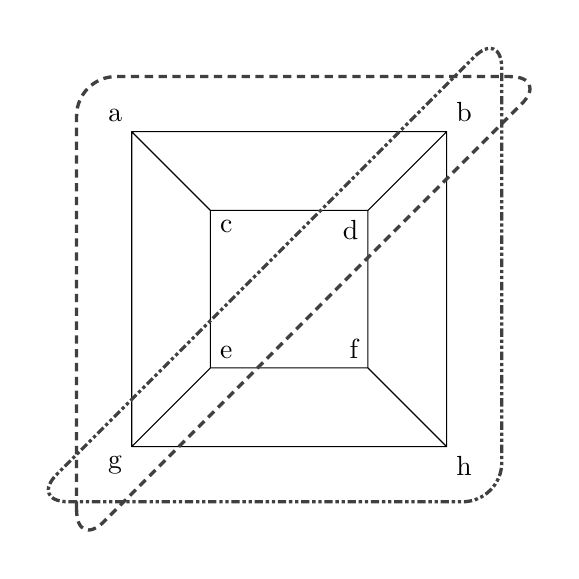
\begin{tikzpicture}[line join=round]
      \draw
        (0,0) node[below left] {g} -- (0,4) -- (1,3) node[below right] {c} -- (1,1) -- cycle
        (0,4) node[above left] {a} -- (4,4) -- (3,3) node[below left] {d} -- (1,3) -- cycle
        (4,4) node[above right] {b} -- (4,0) -- (3,1) node[above left] {f} -- (3,3) -- cycle
        (4,0) node[below right] {h} -- (0,0) -- (1,1) node[above right] {e} -- (3,1) -- cycle;
      \filldraw
        (0,0) circle[] (1,3) circle[]
        (0,4) circle[] (3,3) circle[]
        (4,4) circle[] (3,1) circle[]
        (4,0) circle[] (1,1) circle;
      \draw[very thick, densely dashed, darkgray, rounded corners=5mm]
        (-.7,-1.3) -- (-.7,4.7) -- (5.3,4.7) -- cycle;
      \draw[very thick, densely dash dot dot, darkgray, rounded corners=5mm]
        (-1.3,-.7) -- (4.7,-.7) -- (4.7,5.3) -- cycle;
    \end{tikzpicture}
  }
  \qquad
  \subcaptionbox{
    The tree corresponding to the decomposition in Figure~\ref{fig:decomposition:graph} consists of two vertices.
  }[0.3\textwidth]{
    \begin{tikzpicture}[level distance=1.5cm]
      \node {\{a, b, c, d, e, g\}}
        child {node {\{b, d, e, f, g, h\}}};
      \path (0,-4);  % For alignment
    \end{tikzpicture}
  }
  \caption{
    A tree decomposition of the cube graph of Figure~\ref{fig:graphs:cube}
  }
  \label{fig:decomposition}
\end{figure}

As suggested by the name \enquote{tree decomposition}, trees have an especially interesting decomposition.
In Figure~\ref{fig:decomposition_tree}, it is shown that a tree can be decomposed in such a way that the decomposition mimics the original tree.
\begin{figure}
  \centering
  \subcaptionbox{
    A tree\label{fig:decomposition:tree}
  }[0.4\textwidth]{
    \begin{tikzpicture}
      \draw[text height=2ex, text depth=.5ex]
        (0,0) node[above] {a} -- (-2,-1) node[above left] {b} -- (-3,-2) node[below] {e}
        (0,0) -- (0,-1) node[below] {c}
        (0,0) -- (2,-1) node[below] {d}
        (-2,-1) -- (-1,-2) node[below] {f};
      \filldraw
        (0,0) circle[]
        (-2,-1) circle[] (0,-1) circle[] (2,-1) circle[]
        (-3,-2) circle[] (-1,-2) circle;
      \path (0,-5);  % For alignment
    \end{tikzpicture}
  }
  \qquad
  \subcaptionbox{
    A tree decomposition of the tree in Figure~\ref{fig:decomposition:tree}.
    Observe that the decomposition retains the essence of the structure of the original tree.
    \label{fig:decomposition_tree:decomposition}
  }[0.4\textwidth]{
    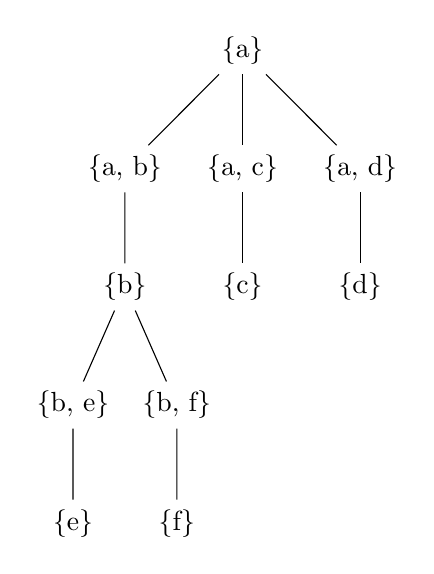
\begin{tikzpicture}[sibling distance=4.25em, level distance=1.5cm]
      \node {\{a\}}
        child {
          node {\{a, b\}}
          child[sibling distance=3.75em] {
            node {\{b\}}
              child {
                node {\{b, e\}} child { node {\{e\}}}
              }
              child {
                node {\{b, f\}} child { node {\{f\}}}
              }
          }
        }
        child {
          node {\{a, c\}} child { node {\{c\}}}
        }
        child {
          node {\{a, d\}} child { node {\{d\}}}
        };
    \end{tikzpicture}
  }
  \caption{
    A tree decomposition of a tree
  }
  \label{fig:decomposition_tree}
\end{figure}
In the tree decomposition in Figure~\ref{fig:decomposition_tree:decomposition} no sets occur with more than two elements.
By the definition of a tree decomposition, any tree decomposition of a graph with at least one edge has a set with at least two elements.
In that sense, the tree decomposition in Figure~\ref{fig:decomposition_tree:decomposition} is optimal.
This leads to the following measure of how much a graph is like a tree.
\begin{definition}
  The \emph{width} of a tree decomposition is the number of elements in the largest set among the vertices of the decomposition, minus one.
  The \defkey{treewidth} of a graph is the least width among the widths of its tree decompositions.
\end{definition}

Indeed, the idea behind the tree decomposition shown in Figure~\ref{fig:decomposition_tree} can be used to prove that the treewidth of any tree with at least one edge is one.
Making sure that trees have a treewidth of one is in fact the reason for the otherwise somewhat peculiar \enquote{minus one} in the definition of the width of a tree.
It follows from Figure~\ref{fig:decomposition} that the treewidth of the cube graph is at most five.
Yet, a tree decomposition of smaller width is possible, as shown in Figure~\ref{fig:decomposition_cube}.
This decomposition happens to be optimal and the treewidth of the cube graph is three.

\begin{figure}[hp]
  \centering
  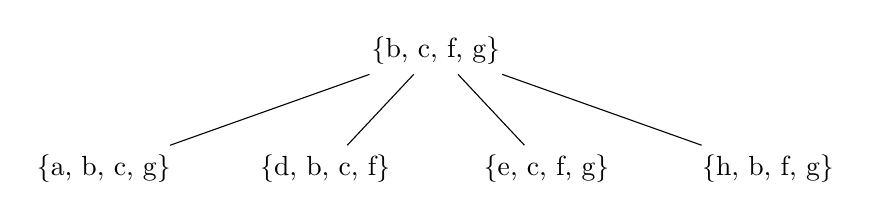
\begin{tikzpicture}[sibling distance=8em, level distance=1.5cm]
    \node {\{b, c, f, g\}}
      child {node {\{a, b, c, g\}}}
      child {node {\{d, b, c, f\}}}
      child {node {\{e, c, f, g\}}}
      child {node {\{h, b, f, g\}}};
  \end{tikzpicture}
  \caption{
    An alternative tree decomposition of the cube graph as shown in Figure~\ref{fig:decomposition:graph}
  }
  \label{fig:decomposition_cube}
\end{figure}

By a fundamental result known as Courcelle's theorem, many graph problems become fixed-parameter tractable once parameterized by treewidth in the \citeauthor{downey1999parameterized} framework~\parencite{downey1999parameterized}.
This includes, for example, \pr{Clique} and \pr{VertexCover}~\parencite{bodlaender2008combinatorial}.
However, the problem of deciding whether the treewidth of an arbitrary graph is less than or equal to a given number is itself \cl{NP}"~complete~\parencite{arnborg1987complexity}.
Therefore, unless \cl{NP} equals \cl{P}, treewidth does not qualify as a parameterization in the framework of \citeauthor{flum2006parameterized}.
At the same time, like with the minimum vertex cover size, computing treewidth is fixed-parameter tractable with respect to itself \parencite[stated in terms of \enquote{branch-width}]{robertson1995graph}.
It is noted by \citeauthor{flum2006parameterized} that large parts of the theory of parameterized complexity go through if we allow for such parameterizations \parencite[279]{flum2006parameterized}.

It has also been recognized that there is little reason why a parameterization should be restricted to only map to a single number~\parencite{fellows2013towards,niedermeier2010reflections}.
A parameterization with a multidimensional image would represent multiple parameters at once.
The interplay between parameters can, however, not be expressed in the \citeauthor{flum2006parameterized} framework.
For example, the minimum vertex cover size of a given graph~$G$ may go down when we remove some of the edges in~$G$.
If we consider the number of edges we remove from a graph and the minimum possible vertex cover size of the resulting graph, we have two interacting parameters.
To bring the minimum vertex cover size down, we need to increase the number of edges we remove.
Note, though, that being allowed to remove an edge need not make it possible to lower the minimum vertex cover size.
We need to remove at least three edges from the cube graph of Figure~\ref{fig:graphs:cube} before the minimum vertex cover size of the graph is no longer four.
It is unclear what a parameterization in the framework of \citeauthor{flum2006parameterized} should map a graph to.
Conceivably, it could map a graph to the \emph{function} that maps the number of modifications performed to the minimum vertex cover size of the resulting graph.
However, this goes against the spirit of fixed-parameter tractability analysis, where we would like to look at specific values for both of our parameters.
On the one hand, the \citeauthor{flum2006parameterized} framework improves on the \citeauthor{downey1999parameterized} framework by separating parameterizations from problems.
It isolates parameterizations as independent objects of study.
On the other, it requires parameter values to be unique for a given instance, which limits its use in analyzing the interplay between different parameters.


\bigsection{Contributions}
\label{sec:contributions}%

This thesis, in Section~\ref{sec:framework}, Section~\ref{sec:tractability:stratified}, and Section~\ref{sec:tractability:order_theory}, introduces a novel take on parameterized complexity theory, rooted firmly in mathematics.
In this new framework, the shortcomings of the two existing frameworks are addressed.
Our contributions are obtained in the five sections of Chapter~\ref{ch:parameterizations}.

We begin an investigation into the extent to which parameterizations can be used as a measure of complexity of individual instances.
A comparison with an older notion of \emph{instance complexity} from algorithmic complexity theory is made in Section~\ref{sec:algorithmic:ic}.
In Section~\ref{sec:algorithmic:randomness_hardness}, a further comparison between instance-based measures of algorithmic and computational complexity is carried out.
A comparison with the notion of \emph{sophistication} from algorithmic statistics is made in Section~\ref{sec:statistics}.

There may be many parameterizations that are of interest for a given problem, so we might hope for the existence of a parameterization that is somehow \emph{optimal}.
In Section~\ref{sec:tractability:optimal} and Section~\ref{sec:tractability:optimalnu}, we provide a near-complete characterization of the problems for which there is an optimal parameterization with respect to fixed-parameter tractability.
We find that there is often no optimal parameterization among those with which a problem is fixed-parameter tractable.

More generally, this thesis furthers our understanding of the class of fixed-parameter tractable problems.
We explore what it means for a problem to be fixed-parameter tractable.
Results of this kind are obtained as a by-product of a more general study of parameterized computability in Section~\ref{sec:computability}.

An alternative characterization of the class of fixed-parameter tractable problems that does not mention parameterizations is suggested in Section~\ref{sec:algorithmic:equivalent_filters}.
In that section, we find out what the parameterizations with respect to which a problem is fixed-parameter tractable tell us about the problem.
We conjecture that the notion of complexity put forth by fixed-parameter tractability is characterized by the quotient group $\Delta^0_1 / \cl{P}$ with respect to symmetric difference.
Here, $\Delta^0_1$ is the class of decidable sets, the first intersection level of the arithmetical hierarchy.

Lastly, in Section~\ref{sec:redundancy}, we uncover a hierarchy inside the class of fixed-parameter tractable problems.
This hierarchy is based on polynomial kernelization, which is a form of reducibility.
